\documentclass[11pt]{article}

\usepackage[letterpaper,margin=1in]{geometry}

% ToC
\usepackage{blindtext} 
\usepackage[linktocpage]{hyperref}
\usepackage{bookmark}
\usepackage{titlesec}

% bib
\usepackage[round]{natbib}

% Math Imports
\usepackage{amsmath, amssymb, bm, fancyhdr, sectsty, dsfont, mathtools}

% Tikz
\usepackage{tikz}
\usetikzlibrary{bayesnet}
\usetikzlibrary{arrows}

\usepackage{wrapfig}
\usepackage{comment}
\usepackage{subcaption}

% Symbols
\newcommand\ind{\protect\mathpalette{\protect\independenT}{\perp}}
\def\independenT#1#2{\mathrel{\rlap{$#1#2$}\mkern2mu{#1#2}}}
\newcommand\norm[1]{\left\lVert#1\right\rVert}
\newcommand\set[1]{\left\{#1\right\}}

\newcommand\RNN{\mathrm{RNN}}
\newcommand\MLP{\mathrm{MLP}}
\newcommand\enc{\mathrm{enc}}
\newcommand\softmax{\mathrm{softmax}}

% Distributions
\newcommand{\Cat}{\mathrm{Cat}}
\newcommand\Expo{\mathrm{Expo}}
\newcommand\Bern{\mathrm{Bern}}
\newcommand\Pois{\mathrm{Pois}}
\newcommand\Bin{\mathrm{Bin}}
\newcommand\Unif{\mathrm{Unif}}
\newcommand\Betad{\mathrm{Beta}}
\newcommand\Gammad{\mathrm{Gamma}}
\newcommand\Geom{\mathrm{Geom}}
\newcommand\Logd{\mathrm{Logistic}}

\newcommand\E[1]{\mathbb{E}\left[#1\right]}
\newcommand\Es[2]{\mathbb{E}_{#1}\left[#2\right]}
\newcommand{\Var}{\mathrm{Var}}
\newcommand{\Cov}{\mathrm{Cov}}
\newcommand{\Cor}{\mathrm{Cor}}

% Bold stuff
\newcommand{\ba}{\mathbf{a}}
\newcommand{\bb}{\mathbf{b}}
\newcommand{\bc}{\mathbf{c}}
\newcommand{\bd}{\mathbf{d}}
\newcommand{\be}{\mathbf{e}}
\newcommand{\bg}{\mathbf{g}}
\newcommand{\bh}{\mathbf{h}}
\newcommand{\br}{\mathbf{r}}
\newcommand{\bs}{\mathbf{s}}
\newcommand{\bw}{\mathbf{w}}
\newcommand{\bx}{\mathbf{x}}
\newcommand{\by}{\mathbf{y}}
\newcommand{\bz}{\mathbf{z}}

% mathcal stuff
\newcommand{\mcD}{\mathcal{D}}

% math blackboard bold stuff
\newcommand{\R}{\mathbb{R}}
\newcommand{\C}{\mathbb{C}}
\newcommand{\Z}{\mathbb{Z}}
\newcommand{\N}{\mathbb{N}}
\newcommand{\Q}{\mathbb{Q}}


\DeclareMathOperator*{\argmin}{argmin}
\DeclareMathOperator*{\argmax}{argmax}

\usepackage{fancyhdr}

\begin{document}
\lhead{Justin Chiu}
\chead{2018 NSF GRFP}
\rhead{Research Proposal}

\section{Introduction}
\subsection{ideas}
Why should we care about text generation?

Story:
In the early 2000's we had modular probabilistic models,
but the focus was on information extraction and alignment.
Now that we have powerful language models and classification methods,
the focus has instead shifted to text generation.
However the shift towards language modeling has de-emphasized the role of
modularity in modeling and resulted in large black-box models with little structure. 
\citep{wiseman2017d2t}

Past work ie \citep{liang2009semalign} modular approach
Current: blackbox throw everything into the language model
\citep{wiseman2017d2t}
Talk about the evaluation metrics, CO, CS, Realization?
And how that inspires a generative model

\begin{enumerate}
\item Controllable, discourse-level features?
Or more like just program induction-y structure
\citet{rabinovich17codegen}
\item Hierarchical generation with weak supervision enforced through posterior regularization
\citep{ganchev2007empc,graca2010pralign,ganchev2010posteriorregularization}
\item Learning higher order features of data table
\item Also, examine the effect of explaining away on fidelity of
generations to underlying records (via noisy channel)
\citep{klein2002conditional,yu2016noisychannel,brown1993mt}
\end{enumerate}

\subsection{real}

We aim to increase the modularity of our probabilistic model in order to leverage weak supervision
\citep{ganchev2010posteriorregularization}.

An open question in language generation is how to incorporate weaker forms of supervision.
Modular graphical models offer a principled way of incorporating weak or indirect supervision
through posterior regularization \citep{ganchev2007empc,graca2010pralign,ganchev2010posteriorregularization}.

Neural network-based language models have achieved top performance \citep{yang2017moslm},
allowing text generation models to become proficient at
generating short snippets of fluent text in applications such as translation \citep{bahdanau2014mt}.
Recent work in language generation has largely relied on the strong language modeling capabilities
of neural models \citep{wiseman2017d2t},
while slowly returning to the modularity afforded by probabilistic models \citep{wiseman2018template,deng2018vattn}.
However, in leveraging powerful language models,
the field's focus has shifted from information extraction to generation as the (conditional)
language modeling capabilities of neural networks have allowed models to learn fluency.

Goals:\citet{wiseman2017d2t}, \citep{liang2009semalign}
\begin{itemize}
\item If we remove burden from the language model, will it lie less?
Only have the LM focus on fluency
\item Having a more structured model paves the way for more interpretable and
modular additions to the system, such as numerical comparisons or list modules
\end{itemize}

% Maybe goal is to demonstrate the modularity of probabilistic models?
% Need to also compare to soft model
% Result might just be that it present a different inductive bias

We would like to incorporate the modularity of a probabilistic framework into the powerful 
autoregressive modeling capabilities of a neural language model.
Although the approach brought only marginal benefits in \citet{deng2018vattn},
it can potentially be applied in many other domains. 
Alignment in translation allows models to properly condition on the source.

% Concerned with jointly learning a generative model and information extraction system.
% Is there an efficiency gain in using the approximate posterior as
% a separate system rather than finding viterbi best alignments?

\section{Problem}
We would like to learn a conditional model
over sentences $\by = \{y_0, y_1, \ldots\}$ and latent structure $\bz$ given a table $\bx$.
We are primarily interested in the respective conditional distributions:
both the posterior distribution over structure given a sentence and table $p(\bz\mid\by,\bx)$,
as well as the conditional distribution over summaries
$p(\by\mid\bx)=\Es{\bz\sim p(\bz\mid\bx)}{p(\by\mid\bz,\bx)}$.
Note that the posterior distribution over structure $p(\bz\mid\by,\bx)$
is an information extraction model.

\section{Related Work}
% Information Extraction methods
\citet{liang2009semalign} also use a conditional model of utterances and use a similar model of alignment.
However, their model is more concerned with using the posterior for information extraction and 
alignment with a database rather than both text generation as it does not include a language model. 
Instead the words are modeled independently from each other given the underlying record structure.

% Generation Methods
The model in \citet{wiseman2017d2t} uses a conditional language model with a copy mechanism
to model summaries given a list of records.
Although the resulting generations are quite fluent, they are not
as faithful to the underlying table as baseline template models which copy from
records deterministically.

% Unsupervised Typing
The model of \citet{rabinovich17codegen}, used for code generation and semantic parsing,
has a very similar flavour.
It assumes a similar underlying generative process, although the conditioning is different:
to produce a program given a natural language statement,
first decide which class of constructor to use then recursively fill in the fields.
However, in our model we are not given pre-specified constructor classes and
we do not have recursive expressions.

% Hierarchical Model
Although the hierarchical model in \citet{yarats2017dialogue} is a HSMM,
the domain and training method are quite different?
Also not doubly hierarchical. %LMAO

\section{Data to Document}
The copy models in \citet{wiseman2017d2t} are trained independently from the
information extraction model. 
The copy model is trained by generating the summary conditioned on the full table.
The information extraction model used for evaluation is trained using labels
created by comparing tokens in the summary with the entities and values from the database.
See \citet{wiseman2017d2t} for all the tricks used in training the model.

Our goal is to use more structure in our model in order to unburden the language model
and prevent hallucination of facts.

We assume that every sentence has an implicit labelling or cluster.

\subsection{The Model}
Let $y_t$ be the current token, $\by_{0:t-1}$ all previous tokens,

\begin{figure}[ht]
\centering
\begin{subfigure}[]{0.3\textwidth}
\centering
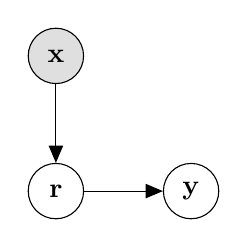
\begin{tikzpicture}
\node(x)[obs]{$\bx$};
\node(r)[latent, below =of x]{$\br$};
\node(y)[latent, right =of r]{$\by$};
\edge {x} {r};
\edge {r} {y};
\end{tikzpicture}
\caption{}
\end{subfigure}

\hspace{0.03\textwidth}
\begin{subfigure}[]{0.3\textwidth}
\centering
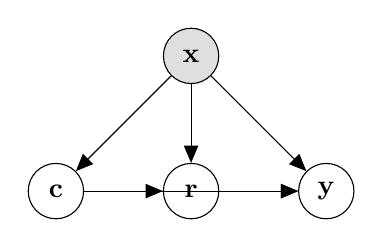
\begin{tikzpicture}
\node(x)[obs]{$\bx$};
\node(r)[latent, below =of x]{$\br$};
\node(c)[latent, left =of r]{$\bc$};
\node(y)[latent, right =of r]{$\by$};

\edge {x} {c};
\edge {x} {r};
\edge {x} {y};
\edge {c} {r};
\edge [bend right=45] {c} {y};
\edge {r} {y};

\end{tikzpicture}
\caption{}
\end{subfigure}
\hspace{0.03\textwidth}

\begin{comment}
% Noisy channel model
\begin{subfigure}[]{0.3\textwidth}
\centering
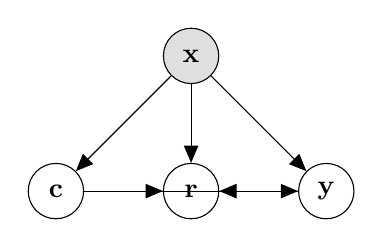
\begin{tikzpicture}
\node(x)[obs]{$\bx$};
\node(r)[latent, below =of x]{$\br$};
\node(c)[latent, left =of r]{$\bc$};
\node(y)[latent, right =of r]{$\by$};

\edge {x} {c};
\edge {x} {r};
\edge {x} {y};
\edge {c} {r};
\edge [bend right=45] {c} {y};
\edge {y} {r};
\end{tikzpicture}
\caption{}
\end{subfigure}
\end{comment}

\begin{subfigure}[]{0.3\textwidth}
\centering
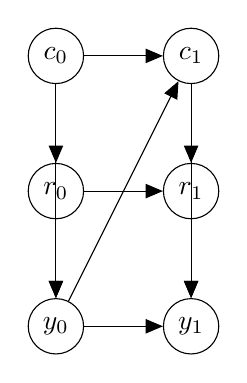
\begin{tikzpicture}
\node(c0)[latent]{$c_0$};
\node(r0)[latent, below =of c0]{$r_0$};
\node(y0)[latent, below =of r0]{$y_0$};
\node(c1)[latent, right =of c0]{$c_1$};
\node(r1)[latent, below =of c1]{$r_1$};
\node(y1)[latent, below =of r1]{$y_1$};

\edge {c0} {r0};
\edge [bend right=45] {c0} {y0};
\edge {r0} {y0};

\edge {c1} {r1};
\edge [bend left=45] {c1} {y1};
\edge {r1} {y1};

\edge {c0} {c1};
\edge {r0} {r1};
\edge {y0} {y1};

\edge {y0} {c1};

\end{tikzpicture}
\caption{}
\end{subfigure}
\label{fig:dgm}
\caption{Simplistic directed graphical models for the latent variable model.
The observed context is $\tilde\bx$, current attention $a_t$, previous attention $a_{t-1}$,
state $s_t$, and target word $y_t$.}
\end{figure}

\begin{figure}[ht]
\label{fig:dgm2}
\caption{The time-series graphical model.
As all nodes condition on $\bx$, we omit it from the diagram.}
\end{figure}

\section{Generative Model}
We present a conditional model that is an extension of \citet{liang2009semalign}'s
simple model that incorporates a neural language model.

Given that many sentences can be clustered into classes, for example
many sentences list a single player's statistics during the game or 
compare the final scores of the two teams and proclaim a winner,
we propose to model a super-segmentation of groups of records with a HSMM,
where each text is then generated from records via another HSMM.
We first make the simplifying assumption that a super-segmentation is a sentence.

\begin{description}
\item[Class choice]
We start with a model over segment classes $p(c_t\mid c_{t-1},y_{t-1},\bx)$,
where we transition to a new class if $y_{t-1}$ is the end of sentence token:
$$p(c_t\mid c_{t-1},y_{t-1},\bx) = \begin{cases}
c_t & y_{t-1}=\textrm{eos}\\
p(c_t\mid c_{t-1},\bx) & \textrm{otherwise}
\end{cases}$$
We could potentially use a fully connected model if we are willing to sacrifice
exact inference $p(c_t\mid \bc_{<t}, \bx)$, which would be realized by a neural
language model over segment classes.
Actually, if we use again use a soft model over $\bc_{<t}$ we can do this tractably,
i.e. use the filtered marginals as input to an RNN:
$p(z_t=i\mid z_{t-1}=j; \E{\bz_{<t-1}}) = \textrm{softmax}(i * \textrm{RNN}(j, \E{\bz_{<t-1}}))$.
We model the initial distribution over classes $\pi(c_0\mid\bx)$
via a neural network over the list of records.
\item[Record choice]
We begin with a markov model over records as in \citet{liang2009semalign} $p(r_t\mid r_{t-1},c_t,\bx)$.
$p(r_{t,i}\mid\br_{t,<i},c_t,\bx)$
\item[Token choice]
$p(y_{t,i,j})\mid\by_{t,i,<j},\by_{t,<i},r_{t,i})$
\end{description}
the first is assume that words $y_t$ are aligned to either a subset of records in $r_{0:N}$ or a null record
recall that a record is a tuple of type {ie POINTS}, entity {Jason Kidd}, value {19}

so given that subset we could then parameterize a categorical distribution over its elements.
let $p(pi | c, r_{0:N})$ be a distribution over binary masks ${0,1}^N$. 
we could decompose $p(r_t | c_t, r_{0:N}) = p(r_t | pi(r_{0:N})) * p(pi | c, r_{0:N})$,
where we would then use posterior regularization: train $p(pi | c, r_{0:N})$ to match
$\textrm{findRecord}(y_t)$ and learn
$p(r_t | pi(r_{0:N}))$ through max marginal likelihood using $\textrm{findRecord}(y_t)$ to give us $\pi$.

\section{Information Extraction Model}
Recall the information extraction model from \citet{wiseman2017d2t}.
$q$

\subsection{Table Completions: Learning Conjunctions}
Introduce latent variables $\bh_i\sim\Bern(\theta_i),i\in\set{0,\ldots,K}$
where $K$ is a hyperparameter. 

\subsection{Noisy Channel?}
Introduce latent variable $\bh$ and 

\section{Training and Inference}
To start, we let $q(\bz\mid\by,\bx)$ take the form of a
delta function take the form of a segmentation.
$$q(z_t\mid\by,\bx)=$$
we can align every word $y_t$ by looking at every record $r_{0:N}$ and checking if $y_t$ matches $r_i.entity$ or $r_i.value$
so let
$$\textrm{findRecord}(y_t) = \set{ r_i \mid r_i.entity = y_t OR r_i.value = y_t }$$
\subsection{Approximate Posterior or Posterior Regularization?}

\section{Related Work}

\section{Results}

\section{NSF STUFF}
\section{Background}
Separate content from style
\section{Research Question}

\section{Keywords}
\section{Approach and Methods}
\section{Intellectual Merit}
\section{Broader Impact}


\bibliographystyle{plainnat}
\bibliography{w}

\end{document}

